\documentclass[usenames,table,dvipsnames,aspectratio=169]{beamer}
% \documentclass[table]{beamer}
\usepackage[utf8]{inputenc}
\usepackage[spanish]{babel}
\usepackage{beamerthemeshadow}
\usepackage{times}
\usepackage{graphicx}
\usepackage{amsmath,amssymb,amsfonts,latexsym,stmaryrd}
\usepackage{tabularx}
\usepackage{xcolor}
\usepackage{color, colortbl}
\usepackage{tikz}
\usepackage{shadow} 
\usepackage{listings}
\usepackage{multirow}
\usepackage{rotating}
\usepackage{../res/lstlangarm}
\usepackage{../res/mips}
\usepackage{ragged2e} % para justificar texto
\usepackage{siunitx}
\usepackage[absolute,overlay]{textpos}
\usepackage{fontawesome5}
\usepackage{pifont}
\usepackage[most]{tcolorbox}

\setbeamertemplate{navigation symbols}{}


\graphicspath
{
{../img/}
}

\usetikzlibrary{calc}
\pgfdeclarelayer{background}
\pgfdeclarelayer{foreground}
\pgfsetlayers{background,main,foreground}

\newcommand{\arm}{\textbf{\textit{arm}}}
\newcommand{\Thumb}{\textbf{\textit{Thumb}}}
\newcommand{\Thdos}{\textbf{\textit{Thumb-2}}}
\newcommand{\jazz}{\textbf{\textit{Jazelle}}}
\newcommand{\tbee}{\textbf{\textit{ThumbEE}}}


\mode<presentation>{
	\usetheme{Copenhagen}
	\useoutertheme{infolines}

}
\setbeamercovered{invisible}
\setbeamercovered{%
  again covered={\opaqueness<1->{1}}}
\parskip=1ex

\title{Procesadores ARM}

\author{Alejandro Furfaro}
\date{\today}

\begin{document}

\lstset{
	frame=Ltb,
	framerule=0pt,
	aboveskip=0.5cm,
	framextopmargin=3pt,
	framexbottommargin=3pt,
	framexleftmargin=0.4cm,
	framesep=0pt,
	rulesep=.4pt,
	backgroundcolor=\color{gray97},
	rulesepcolor=\color{black},
	language=[ARM]Assembler,
	captionpos=b,
	tabsize=6,
	frame=lines,
	keywordstyle=\color{blue},
	commentstyle=\color{purple},
	stringstyle=\color{red},
	numbers=left,
	numberstyle=\tiny,
	numbersep=5pt,
	breaklines=true,
	showstringspaces=false,
	basicstyle=\small,
	emph={label},
	framerule=0pt,
}

\begin{frame}[plain]{Procesadores ARM. Arquitectura ARMv7}
  \begin{figure}[h]
  \centering
  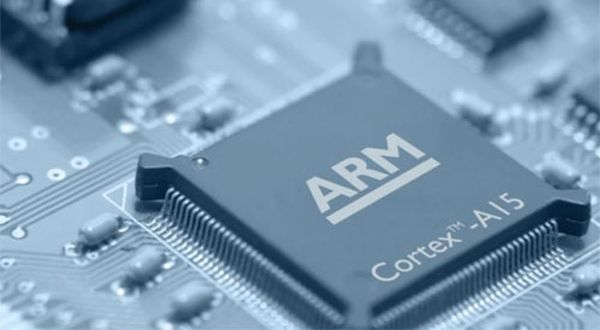
\includegraphics [width =0.6\textwidth]{ARM-Cortex.jpg}
\end{figure}
\vspace{-2cm}
\titlepage
\end{frame}

\AtBeginSubsection[]
{
\begin{frame}{Temario}
\begin{textblock*}{\textwidth}(0.4cm,1.5cm)
%   \begin{multicols}{2}
    \setcounter{tocdepth}{2}  
    \footnotesize \tableofcontents[currentsection, currentsubsection, sectionstyle=show/shaded, subsectionstyle=show/shaded]
%   \end{multicols}
\end{textblock*}
\end{frame}
}

\begin{frame}{Temario}
\begin{textblock*}{\textwidth}(0.4cm,1.5cm)
%  \begin{multicols}{2}
  \footnotesize \tableofcontents
%  \end{multicols}
\end{textblock*}
\end{frame}



\definecolor{OliveGreen}{RGB}{2,80,1}
\definecolor{LigthOrange}{RGB}{255,255,200}
\definecolor{gray97}{gray}{.97}
\definecolor{Gray}{RGB}{171,174,178}
\definecolor{orange}{RGB}{255,127,0}


\section{ARM: Advanced RISC Machines}
\subsection{Introducción}

\begin{frame}{Un Modelo de Negocio muy original}
 \begin{textblock*}{\textwidth}(.3cm,1.2cm)
  \begin{itemize}[<+(1)->] \justifying \parskip 0.3cm
   \item ARM1: primer procesador creado por Acorn Computer en 1985. Apuntaba al mercado desktop (dominado por Intel y Motorola).
   \item Evoluciona en ARM2 y ARM3. Los únicos nichos eran educación, y hobbistas fundamentalmente.
   \item Aparecen empresas interesada en integrar procesadores ARM en sus propios diseños de sistemas embebidos. En especial Apple.
   \item Nace Advanced RISC Machine (ARM), producto del aporte de capital de Apple y know how e ingeniería de Acorn.
   \item Su modelo de negocios será diferente del clásico. \textit{En lugar de vender el chip con el procesador, vende los derechos de propiedad intelectual para que otras compañías empleen procesadores ARM en sus diseños embebidos}.
  \end{itemize}
\end{textblock*}
\end{frame}

\begin{frame}{1er. Hito ARM7TDMI (1993)}
 \begin{textblock*}{.5\textwidth}(.3cm,1.2cm)
  \begin{enumerate}[<+(1)->]
   \item Lanzado en 1993
   \item Fue el procesador elegido por Apple para el iPod.
   \item \textbf{\textit{D}} por \textbf{D}ebug Interface.
   \item \textbf{\textit{I}} por \textbf{I}CE o In Circuit Emulation
   \item \textbf{\textit{M}} por \textbf{M}ultiplier (incluido en el datapath).
   \item Set de instrucciones \Thumb
   \item pipeline de tres etapas
  \end{enumerate}
 \end{textblock*}
 \begin{textblock*}{.5\textwidth}(.53\textwidth,1.2cm)
  % \begin{onlyenv}<8-8>
   \centering \includegraphics<8->[width=\textwidth]{ARM7TDMI-pipeline.png}
  % \end{onlyenv}
 \end{textblock*}
\end{frame}

\begin{frame}{ARM7TDMI - Diagrama}
 \begin{columns}[onlytextwidth, T]
  \begin{column}{.38\textwidth}
   \centering 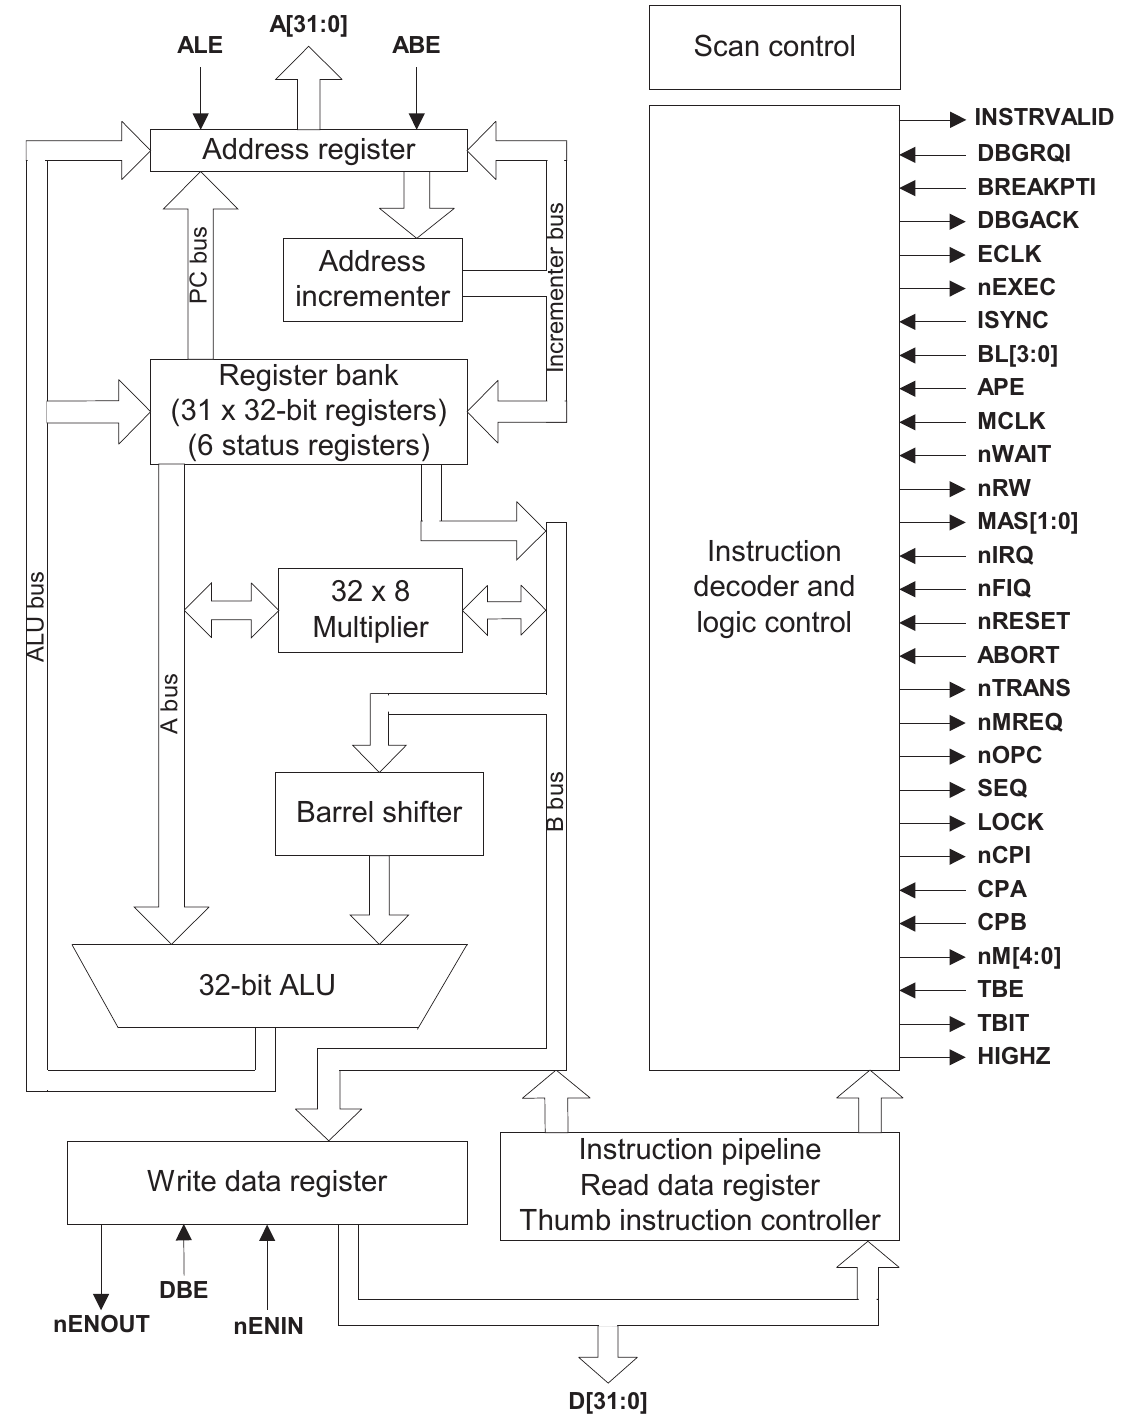
\includegraphics[width=\textwidth]{ARM7TDMI-diagrama.png}
  \end{column}
  \begin{column}{.57\textwidth}
   \begin{itemize}[<+(1)->] \justifying
    \item Claramente modelo Von Newmann
    \item 6 Modos de Operación.
    \item 37 registros. Pero en cada momento hay 16 visibles
    \item Incluye Multiplicación\dots ¿Como? ¿No era RISC?
    \item El Modo \Thumb{ } fué altamente adoptado a medida que este procesador empezó a utilizarse en los teléfonos móviles para economizar memoria.
    \item A pesar de su éxito comercial por el iPod no pasa de un Microcontrolador. No soporta sistemas de Propósito general,
  \end{itemize}
 \end{column}
 \end{columns}
\end{frame}

\begin{frame}{ARM - Genealogía}
 \begin{textblock*}{.7\textwidth}(0.4cm,1.2cm)
  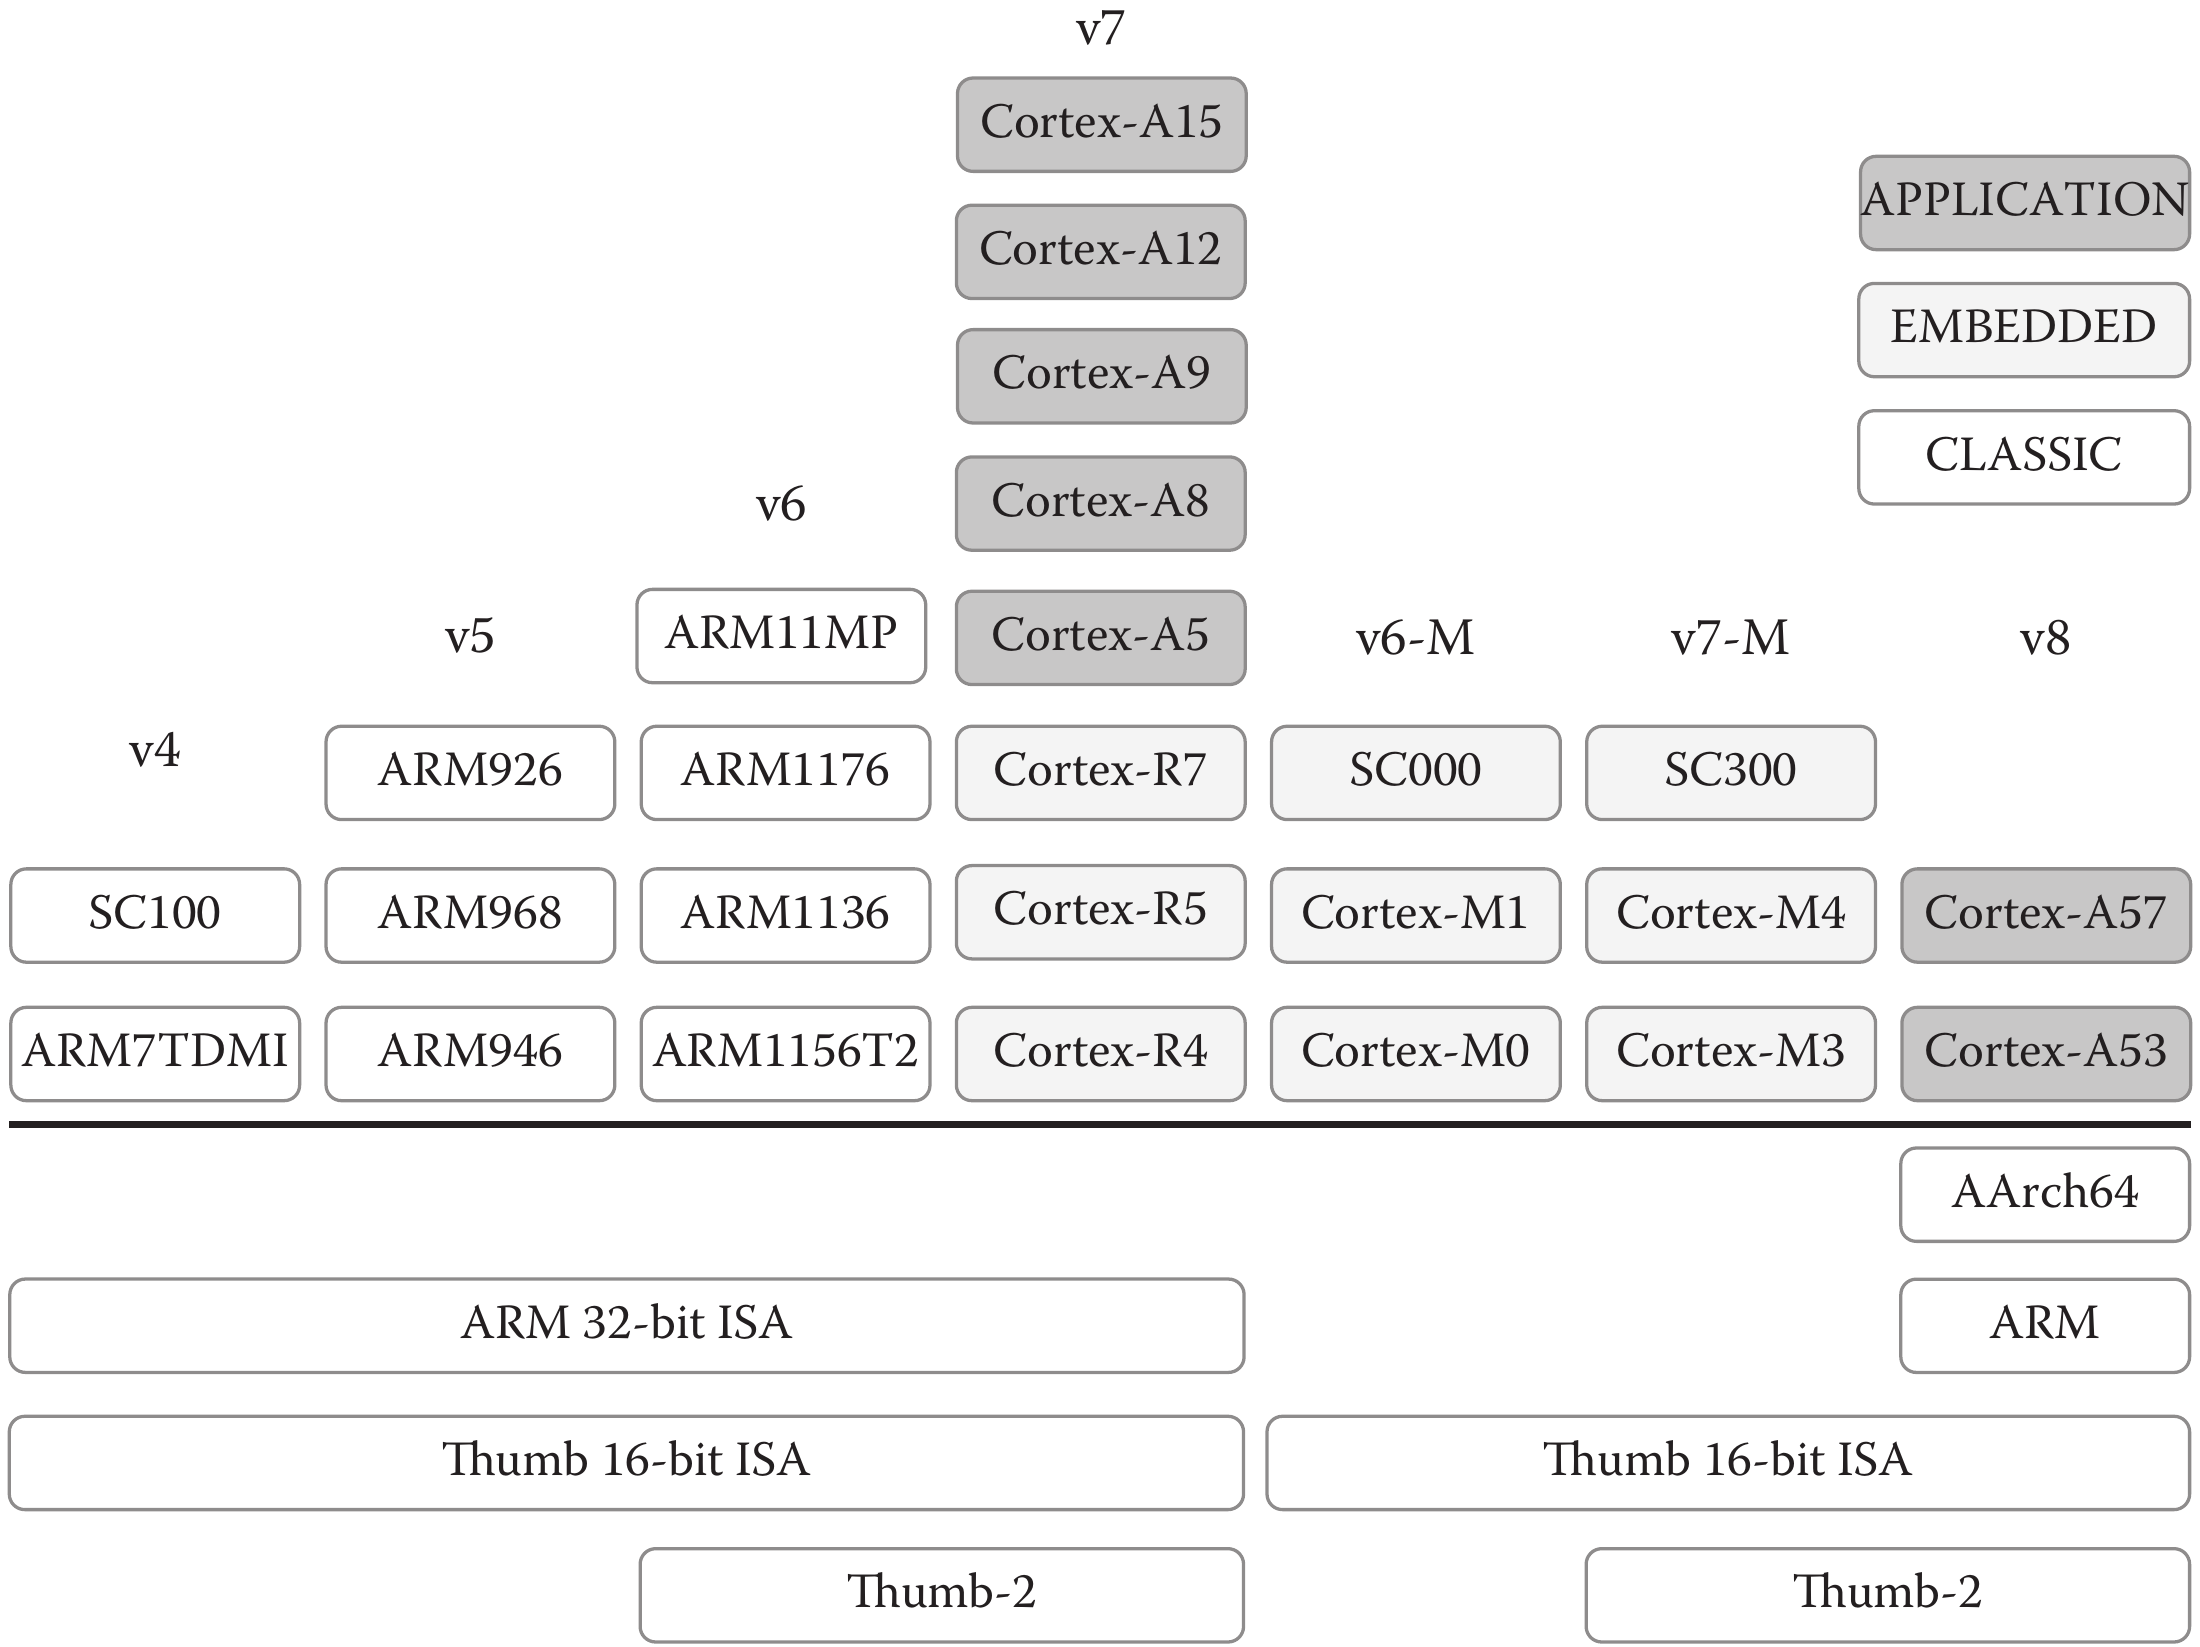
\includegraphics[width=.85\textwidth]{ARM-genealogia.png}\\
    \centering Evolución de versiones de Arquitectura
 \end{textblock*}
  \begin{textblock*}{.4\textwidth} (\dimexpr0.4cm + .6\textwidth\relax, 1.2cm)
   \begin{itemize}[<+(1)->]\justifying
    \item En algo mas de 20 años se transformó una arquitectura de microcontrolador en una de procesador serio.
    \item No esperen milagros.
    \item Para quienes creen que con Intel lo han visto todo en materia extravagancias y falacias técnicas de diseño\dots
    \item Preparen pop corn...
   \end{itemize}
  \end{textblock*}
\end{frame}

\section{Arquitectura}
\subsection{Secciones importantes}
\begin{frame}{Arquitectura Cortex-A y CORTEX-R}
 \begin{textblock*}{\textwidth}(.3cm,1.2cm)
  \begin{block}<1->{Objetivos de la ARMv7}
   \justifying De la lectura de las primeras páginas de ``ARM Architecture Reference Manual, ARMv7-A and ARMv7-R Edition'', puede notarse que ARM se propone definir los aspectos arquitecturales de procesadores RISC que sean capaces de implementar un amplio rango de soluciones mediante sistemas de pequeño tamaño, lo cual produce un consumo los mas bajo posible, manteniendo niveles de performance aceptables. Si lo logra o no será materia de análisis luego de experimentar lo suficiente. 
  \end{block}
  \begin{itemize}[<+(1)->] \justifying
   \item Set de 16 Registros de Propósito General (Solo 13 son realmente de propósito general, como veremos).
   \item Acceso a memoria Load / Store. (Los operandos de instrucciones aritmético lógicas son Registros).
   \item Los Modos de direccionamiento de memoria son relativamente simples. Utilizan de registros índices, y/o desplazamientos inmediatos.
  \end{itemize}
 \end{textblock*}
\end{frame}

\begin{frame}{Arquitectura Cortex-A y Cortex-R}
 \begin{textblock*}{\textwidth}(.3cm,1.2cm)
  \begin{itemize}[<+(1)->] \justifying \parskip .4cm
   \item Tiene instrucciones que combinan desplazamientos con operaciones aritméticas y lógicas.
   \item Auto incremento/decremento de direcciones en instrucciones de acceso a memoria para optimizar loops.
   \item Load/Store Múltiples para optimizar operaciones de acceso a memoria.
   \item Mecanismos para Ejecución Condicional de Instrucciones para acelerar ejecución (para el mundo de los microcontroladores muy interesante pero para procesadores de alta gama irrelevante a la luz de las Unidades de predicción de salto).
  \end{itemize}
 \end{textblock*}
\end{frame}

\begin{frame}{Set de instrucciones}
 \begin{textblock*}{\textwidth}(.3cm,1.2cm)
  \begin{itemize}[<+(1)->]\justifying %\parskip 0.15cm
   \item El set de instrucciones ARM es de \SI{32}{\bit}, tamaño fijo, y campos de operandos también fijo, de acuerdo con los lineamientos RISC.
   \item Con el objetivo de lograr una mayor densidad de código ARM desarrollo un set de instrucciones de \SI{16}{\bit} de tamaño, y lo denominó \textbf{\textit{Thumb}}.
   \item El costo de esta mejora en densidad es la performance.
   \item Por otra parte, \textbf{\textit{Thumb}} es un subset del set original de \SI{32}{\bit} (que se denomina \textbf{\textit{arm}})
   \item En segmentos críticos de código como por ejemplo un handler de interrupción, es posible pasar de maner temporal de ejecutar instrucciones \textbf{\textit{thumb}} a ejecutar instrucciones de \SI{32}{\bit} (\textit{\textbf{arm}})
   \item Luego de ARMv6, ARM presenta la arquitectura ARMv6T2, que introduce la Tecnología \textit{\textbf{Thumb-2}}.
   \item Agrega una serie de instrucciones de \SI{32}{\bit} que permiten aproximar en gran medida la performance con el modo \textbf{\textit{arm}} puro, a la vez que mantiene una baja densidad de código.
  \end{itemize}
 \end{textblock*}
\end{frame}

\begin{frame}{Extensiones}
 \begin{textblock*}{\textwidth}(.3cm,1.2cm)
  \begin{itemize}[<+(1)->]\justifying \parskip 0.3cm
   \item En general los diseñadores de Procesadores RISC al principio utilizan la menor cantidad posible de instrucciones.
   \item En la medida que se busca que este procesador sea mas competitivo dentro de su segmento, se agregan sub sets de instrucciones para enriquecer su capacidad de procesamiento.
   \item Normalmente estos sub sets se conocen como Extensiones de Arquitectura. 
   \item ARM tiene varias. Algunas no han logrado despertar demasiado entusiasmo, otras han sido declaradas obsoletas como \textbf{\textit{ThumbEE}}, y \textbf{\textit{Jazzele}}. Otras son de aplicación creciente.
   \item Claro está\dots si se implementan todas las extensiones, los postulados RISC quedan bastante atrás\dots
  \end{itemize}
 \end{textblock*}
\end{frame}

\begin{frame}{Extensiones para Punto Flotante}
 \begin{textblock*}{\textwidth}(.3cm,1.2cm)
  \begin{itemize}[<+(1)->]\justifying\parskip 0.3cm
   \item Es una prestación obligada para aplicaciones de cálculo avanzado.
   \item No es imprescindible en todos los sistemas. Por eso es razonable que sea una extensión.
   \item Aquí encontramos diferentes extensiones para ARMv7-A y ARMv7-R, respecto de ARMv7-M
   \item Para ARMv7-A y ARMv7-R las versiones VFPv3 y vFPv4 establecen los formatos de datos soportados, y los registros involucrados e instrucciones, que se introducen. Soporta solo Single y Half Precision (no Doble Precision).
   \item Para ARMv7-M las versiones FPv4-SP y VFPv5 definen extensiones mínimas para esta arquitectura en relación a las prestaciones que se implementan en las versiones ARMv7-A y R. Diferencia 100\% arquitectural (Tipos de datos e instrucciones)
  \end{itemize}
\end{textblock*}
\end{frame}

\begin{frame}{Extensiones para DSP}
 \begin{textblock*}{\textwidth}(.3cm,1.2cm)
  \begin{itemize}[<+(1)->] \justifying \parskip 0.3cm
   \item Es muy útil cuando se requiere implementar los algoritmos clásicos de Procesamiento Digital de Señales, para procesar audio, video, o imágenes.
   \item No es imprescindible en todos los sistemas. Por eso es razonable que sea una extensión.
   \item Nuevamente encontramos diferentes extensiones para ARMv7-A y ARMv7-R, respecto de ARMv7-M
   \item Para ARMv7-A y ARMv7-R estas extensiones están muy relacionadas con las versiones VFPv3 y vFPv4 de punto flotante vistas en el slide anterior.
   \item Para ARMv7-M se definen algunas instrucciones que derivan en una implementación mas mas modesta de esta extensión. Nuevamente diferencias arquitecturales.
  \end{itemize}
 \end{textblock*}
\end{frame}

\begin{frame}{Extensiones mas avanzadas}
 \begin{textblock*}{\textwidth}(.3cm,1.2cm)
  \begin{itemize}[<+(1)->] \justifying \parskip 0.3cm
   \item ARMv7 tiene  extensiones avanzadas de arquitectura solo para los perfiles A y R.
   \item Security Extensions.
   \item Multiprocessor Extensions
   \item Large Physical Address Extensions. \textbf{\textit{LPAE}}. Lleva a 40 bits la capacidad de direccionamiento.
   \item Virtualization Extensions. Requiere que estén implementadas Security Extensions, y \textbf{\textit{LPAE}}.
   \item Generic Timer Extensions.
   \item Performance Monitoring Extensions
  \end{itemize}
 \end{textblock*}
\end{frame}

\begin{frame}{Modelo de Memoria}
 \begin{textblock*}{\textwidth}(.3cm,1.2cm)
  \begin{block}<2->{Definiciones de ARMv7 respecto de la memoria}
   \begin{itemize}[<+(2)->]\justifying
    \item Organizada como un espacio flat continuo de $2^{32}$ bytes. Puede considerarse también como un espacio de $2^{30}$ palabras de 32 bits o $2^{31}$ palabras de \SI{16}{\bit}.
    \item La CPU puede generar excepciones ante accesos a datos no alineados.
    \item Tiene capacidad de restringir el acceso de las aplicaciones a determinadas áreas de memoria.
    \item Traducción de dirección virtual a dirección física.
    \item Alterar la interpretación datos de \SI{16}{\bit} o \SI{32}{\bit} entre Little Endian o Big Endian.
    \item Controlar el orden de los accesos, y control de caches
    \item Sincronizar el acceso a memoria cuando se tiene mas de una CPU en el sistema.
   \end{itemize}
  \end{block}
 \end{textblock*}
\end{frame}

\begin{frame}{Dos modelos de programación}
 \begin{textblock*}{\textwidth}(.3cm,1.2cm)
  \begin{block}<1-> \justifying
   Siempre que un procesador moderno implementa un modo de trabajo para las aplicaciones, y otro mas Privilegiado para el Sistema Operativo, o cualquier tipo de software de administración ad-hoc, hay dos modelos de programación diferentes, y entre ambos conforman la arquitectura:
   \begin{itemize}[<+(1)->]\justifying\parskip 0.3cm
    \item Modelo de Programación de Aplicaciones\\
    Se compone de los registros de arquitectura en instrucciones accesibles independientemente del modo de trabajo
    \item Modelo de Programación de Sistemas.\\
    Se compone de los registros e instrucciones del modelo de Programación de Aplicaciones, mas un set de registros e instrucciones que solo pueden ser accedidos por código que ejecuta en nivel privilegiado
   \end{itemize}
  \end{block}
 \end{textblock*}
\end{frame}

\section{Modelo de Programación de Aplicaciones}
\subsection{Instruction Set Architecture}
\begin{frame}{Tipo y Tamaño de datos}
 \begin{textblock*}{\textwidth}(.3cm,1.2cm)
  \begin{itemize}[<+(1)->]
   \item El set de instrucciones soporta en memoria estos tipos de datos y sus tamaños:
   \begin{itemize}
    \item Byte $\rightarrow$ \SI{8}{\bit} (1 byte)
    \item Halfword $\rightarrow$ \SI{16}{\bit} (2 bytes)
    \item Word $\rightarrow$ \SI{32}{\bit} (\SI{4}{\byte})
    \item {\color{red} Doubleword\textbf{*} $\rightarrow$ \SI{64}{\bit} (\SI{8}{\byte})} \color{black}
  \end{itemize}
  \item El set de instrucciones trabaja con los siguientes tipos de datos en los registros de arquitectura
  \begin{itemize}
   \item Punteros de \SI{32}{\bit}.
   \item Enteros Signados o No signados de \SI{32}{\bit}.
   \item Enteros No Signados de \SI{16}{\bit} u \SI{8}{\bit}, en formato zero-extended.
   \item Enteros Signados de \SI{16}{\bit} u \SI{8}{\bit}, en formato sign-extended.
   \item {\color{red} Dos enteros de \SI{16}{\bit} empaquetados en un registro.\textbf{*} }
   \item {\color{red} Cuatro enteros de \SI{8}{\bit} empaquetados en un registro.\textbf{*} } \color{black}
   \item Entero No Signado or Signado de \SI{64}{\bit} mantenido en dos registros de \SI{32}{\bit}.
  \end{itemize}
 \end{itemize}
  \only<15->{\color{red} \textbf{*} Solo ARMv7-A y ARMv7-R}
 \end{textblock*}
\end{frame}

\begin{frame}{Endianess}
 \begin{textblock*}{\textwidth}(.3cm,1.2cm)
  \begin{block}<1->{Layout de un byte en memoria}
   \begin{itemize} [<+(1)->]\justifying
    \item Si queremos almacenar un byte no hay ambigüedades posibles.
    \item Ej: Almacenar el valor 0x8A en la dirección de memoria 0x00E1244D.
   \end{itemize}
  \end{block}
 \end{textblock*}
 \begin{textblock*}{\textwidth}(0cm,3.7cm)
   \centering \includegraphics<4->[width=0.36\textwidth]{Byte.pdf}
 \end{textblock*}
\end{frame}

\begin{frame}{Endianess}
 \begin{textblock*}{\textwidth}(.3cm,1.1cm)
  \begin{block}<1->{Layout de un half word, word o doble word en memoria}
   \begin{itemize}[<+(1)->] \justifying
    \item Cuando representamos un valor de varios bytes el orden en el que éstos se almacenan en memoria no es trivial.
    \item Ej: Tenemos el número 0x7F458096. La dirección de memoria destino es \textbf{n}
   \end{itemize}
  \end{block}
 \end{textblock*}
 \begin{textblock*}{\textwidth}(0cm,3.8cm)
  \only<3>{\centering \includegraphics[width=0.36\textwidth]{endianess-layer1.pdf}\\}
  \only<4>{\centering \includegraphics[width=0.36\textwidth]{endianess-layer2.pdf}\\}
  \only<5->{\centering \includegraphics[width=0.36\textwidth]{endianess-layer3.pdf}}
 \end{textblock*}
 \begin{textblock*}{\textwidth}(0.3cm,8cm)
  \only <6-> {\justifying  \textbf{\textit{CORTEX-A y R manejan ambos Endianess. CORTEX-M solo Little Endian}}}
 \end{textblock*}
\end{frame}

\begin{frame}{Aquí está el dato ``al derecho''}
 \begin{textblock*}{\textwidth}(.3cm,1.1cm)
  \centering 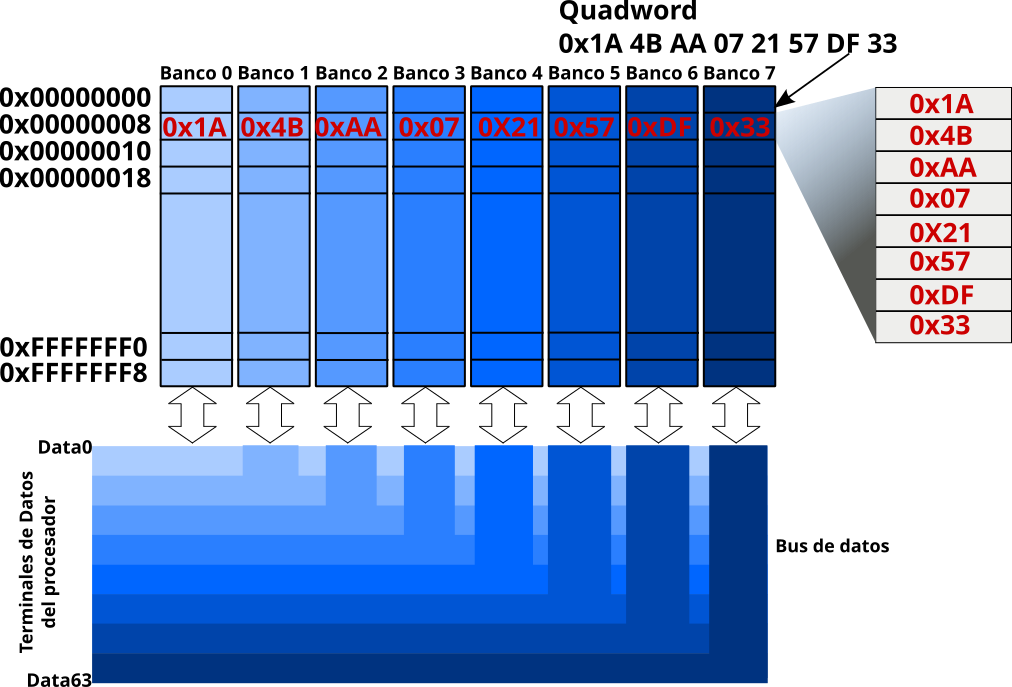
\includegraphics[width=0.7\textwidth]{endianess01.pdf}
 \end{textblock*}
\end{frame}

\begin{frame}{\textquestiondown Estaba de verdad ``al derecho''?}
 \begin{textblock*}{\textwidth}(.3cm,1.1cm)
  \centering 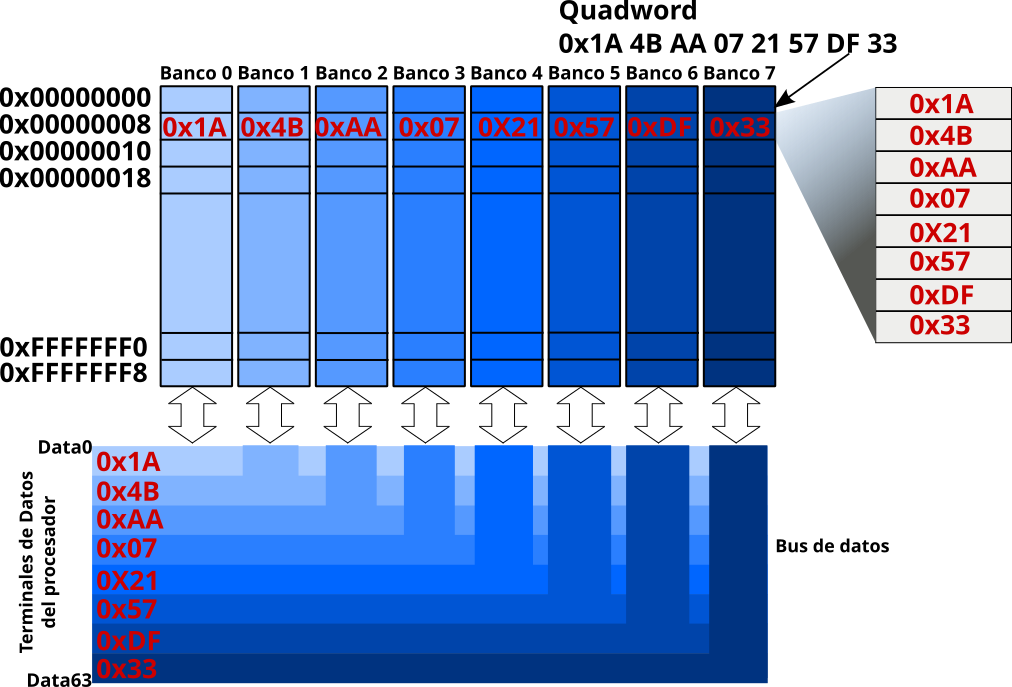
\includegraphics[width=0.7\textwidth]{endianess02.pdf}
 \end{textblock*}
\end{frame}

\begin{frame}{Probemos almacenarlo ``al reves''}
 \begin{textblock*}{\textwidth}(.3cm,1.1cm)
  \centering 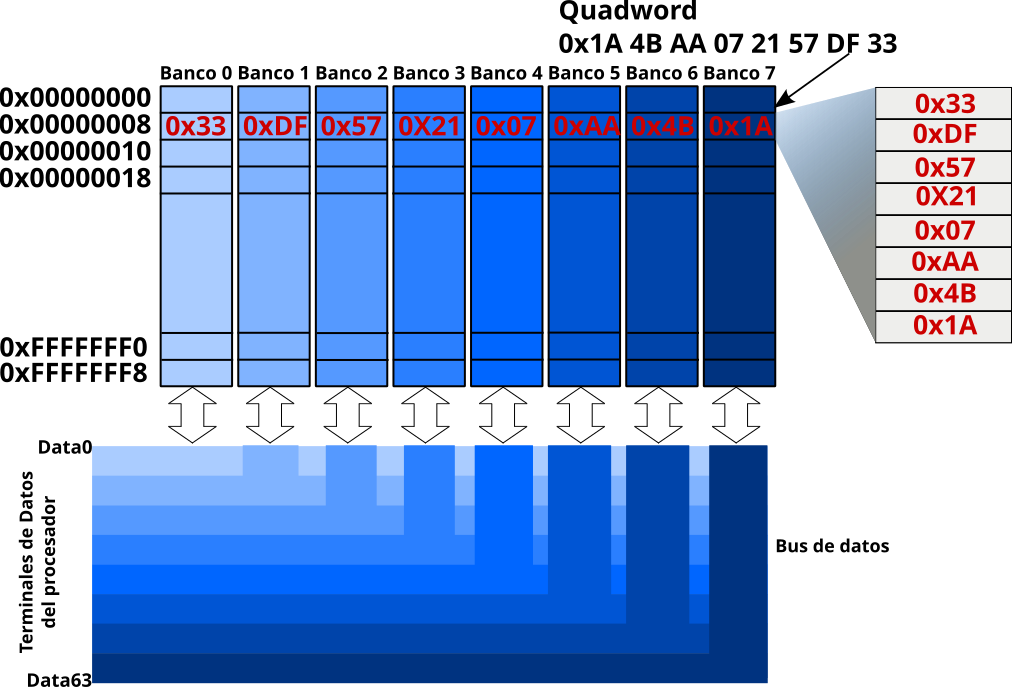
\includegraphics[width=0.7\textwidth]{endianess03.pdf}
 \end{textblock*}
\end{frame}

\begin{frame}[fragile]{llegó ``al derecho'' \dots para la CPU}
 \begin{textblock*}{\textwidth}(.3cm,1.1cm)
  \centering 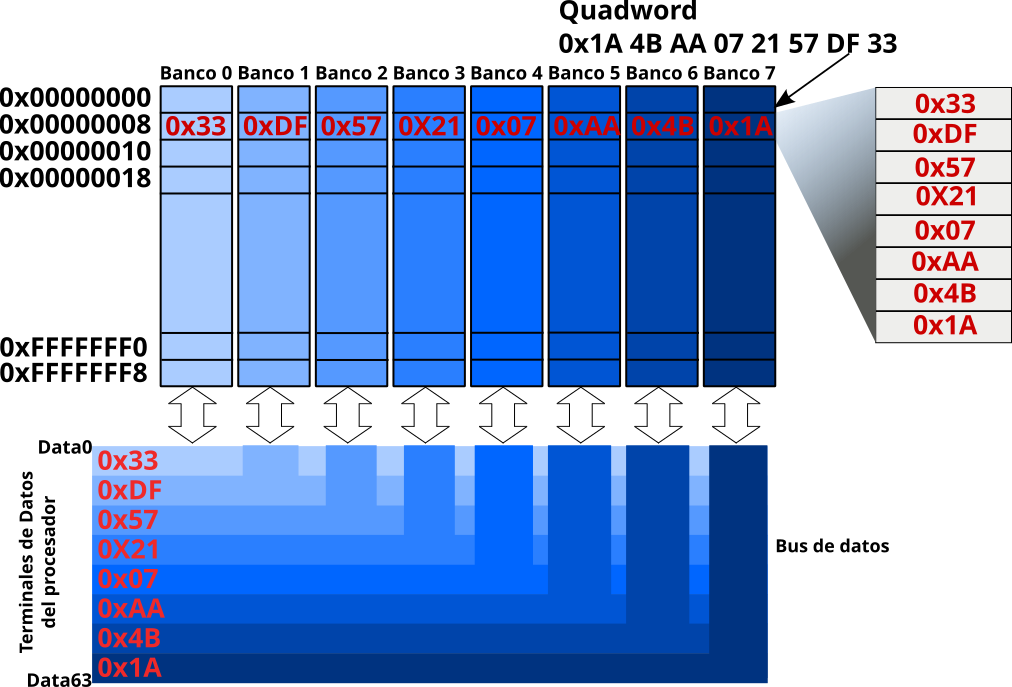
\includegraphics[width=0.7\textwidth]{endianess04.pdf}
 \end{textblock*}
\end{frame}

\begin{frame}{Endianess vs. Hardware}
 \begin{textblock*}{\textwidth}(.3cm,1.1cm)
  \begin{itemize}[<+(1)->] \justifying
   \item El Ingeniero de Hardware define el orden de los bytes que deben llegar al Procesador. Tendecia: Little Endian.
   \item Por default ARM mapea las direcciones en donde busca código en Little Endian, y reserva Endianess configurable para espacios de memoria en donde almacena datos.
   \item El endianness se configura diferente cuando se trata de Sistema Operativo o de aplicaciones:
   \begin{itemize}
    \item \texttt{\textbf{SCTLR.EE}} : endianess de data (privilegiado)
    \item \textbf{\texttt{SCTLR.E0E}}: endianess en user mode (si implementado)
   \end{itemize}
   \item Se asume que estos cambios ocurren durante el early boot, o en su defecto, bajo un contexto muy controlado, o en algún tipo de firmware/secure.
   \item \textbf{\textit{ {\color{orange}\faExclamationTriangle} \color{red} Nunca durante operación normal del OS!}}.
   \item Práctica real:
   \begin{itemize}
    \item Linux / BSD / RTOS fijan endianess al boot, y nunca lo cambian
    \item En ocasiones, los Bootloaders manejan ROM en big-endian y kernel en little-endian. Cambian emdianess \textbf{una sola vez}: antes de saltar al kernel.
   \end{itemize}
  \end{itemize}
 \end{textblock*}
\end{frame}

\begin{frame}{Cambio de Endianess. ``Niños No hagan esos en sus casas!!''}
 \begin{textblock*}{\textwidth}(.3cm,1.1cm)
  \begin{itemize}[<+(1)->] \justifying
   \item Casos donde se cambia (extremadamente poco comunes, y super controlados):
   \begin{itemize}
    \item Compatibilidad con algún bloque legacy big-endian
    \item Firmware que ejecuta código mixto
    \item Hypervisors muy específicos (Extensiones de Vitrualización activas)
    \item Debugging
   \end{itemize}
  \end{itemize}
 \end{textblock*}
\end{frame}

\subsection{Core Registers}
\begin{frame}{Registros de propósito general y dedicados}
 \begin{textblock*}{\textwidth}(.3cm,1.1cm)
  \begin{itemize}[<+(1)->]  \justifying
   \item En el Nivel de Aplicación una CPU ARMv7, presenta 13 registros de propósito general (GPR por General Purpose Register) de \SI{32}{\bit}.
   \item Se llaman \textbf{\texttt{R0}}, \textbf{\texttt{R1}}, \texttt{\textbf{R2}}, ....\textbf{\texttt{R12}}.Tienen la misma funcionalidad todos.
   \item Hay otros tres registros de \SI{32}{\bit} que son en principio registros dedicados:
   \begin{itemize}\justifying
    \item \textbf{SP: Stack Pointer}. Es el registro \textbf{\texttt{R13}}. ARM considera su uso únicamente como puntero a la pila.
    \item \textbf{LR: Link Register}. Es el registro \texttt{\textbf{R14}}. Resguarda la dirección de retorno cuando se invoca un procedimiento (o función), evitando usar la pila. Acelera la ejecución del retorno.
    \item \textbf{PC: Program Counter}. Es el puntero a la próxima instrucción a buscar. En Modo \Thumb{} solo lo modifican los branches. En modo \arm{} lo puede modificar cualquier instrucción {\color{red}\faExclamationTriangle}.
   \end{itemize}
  \item Aunque ARM los incluya en la cuenta como GPR, y los llame \texttt{\textbf{R13}}, \textbf{\texttt{R14}}, y \textbf{\texttt{R15}}... ,son dedicados, indudablemente.
  \end{itemize}
  \only<9> {{\color{blue} \faIcon{search}} \color{black} 1.¿Es sensato modificar el \textbf{PC} con cualquier instrucción?. 2.¿Es \textbf{PC} un registro de propósito general?. 3.¿Y \textbf{SP}?}
 \end{textblock*}
\end{frame}

\subsection{La pila}
\begin{frame}{Funcionamiento básico}
 \begin{columns}[c]
  \column{0.5\textwidth} 
   \begin{figure}[ht!]
	  \centering 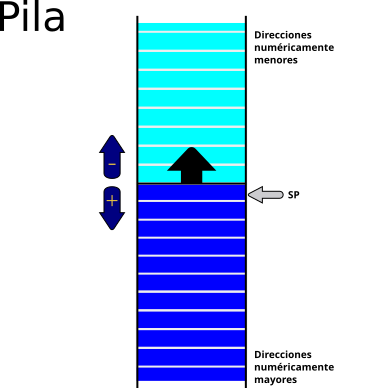
\includegraphics[width=.85\textwidth]{Pila1.pdf}
	 \end{figure}
  \column{0.5\textwidth} 
   \begin{itemize}[<+(1)->]\justifying
	  \item La pila (stack) es un área de memoria contigua, que se maneja como una cola \textbf{LIFO} (\textbf{L}ast \textbf{I}n \textbf{F}irst \textbf{O}ut)
	  \item El tamaño de este bloque puede ser tan grande como se necesite.
	  \item El bloque de memoria se recorre mediante un registro de propósito general, denominado habitualmente en forma genérica stack pointer, y que en los procesadores ARM es el \textbf{\texttt{R13}} o \textbf{\texttt{SP}} cuyo tamaño es de \SI{32}{\bit}.
   \end{itemize}
 \end{columns}
\end{frame}


\begin{frame}{Funcionamiento básico}
 \begin{textblock*}{\textwidth}(.3cm,1.2cm)
  \centering 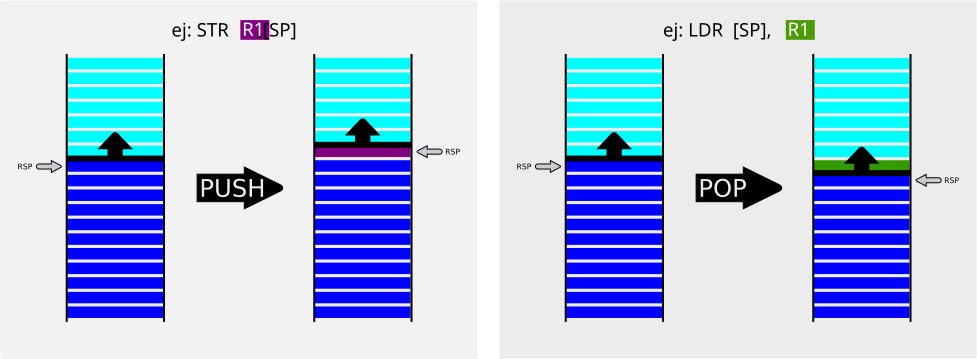
\includegraphics[width=.78\textwidth]{Pila2.pdf}
 \end{textblock*}
 \begin{textblock*}{\textwidth}(.3cm,5.3cm)
  \begin{itemize}[<+(1)->] \justifying
    \item La Operación de guardar un dato en una pila se denomina genéricamente \textbf{PUSH}, y la de retirarlo \textbf{POP}.
    \item Cuando realiza una operación \textbf{PUSH}, el procesador decrementa el registro \texttt{\textbf{SP}} y luego escribe el dato en la pila, en la dirección apuntada por el registro \texttt{\textbf{SP}}.
    \item Cuando realiza una operación \textbf{POP}, el procesador lee el ítem apuntado por el registro \texttt{\textbf{SP}}, y luego incrementa éste último registro.
  \end{itemize}
 \end{textblock*}
\end{frame}


\subsection{Set de Instrucciones}
\begin{frame}{Generalidades}
 \begin{textblock*}{\textwidth}(.3cm,1.2cm)
  \begin{itemize}[<+(1)->]\justifying \parskip 0.15cm
   \item Instrucciones de tamaño fijo (RISC). 32 bits en estado \arm. Se ejecutan en un solo ciclo de clock
   \item Arquitectura Load/Store (RISC)
   \begin{itemize}
    \item No se manipula de manera directa el contenido de la memoria
    \item Los datos en memoria se llevan a la CPU se procesan utilizando los registros, y luego se regresan los resultados a la dirección apropiada de memoria.
   \end{itemize}
   \item Los Cores pueden estar en estado \arm{} o \Thumb.
   \begin{itemize}
    \item Esto determina que set de instrucciones se está utilizando
    \item La transición entre ambos estados es por software (Instrucciones específicas)
   \end{itemize}
   \item Ejecución condicional (reduce el uso de branching en organizaciones simples de microcontrollers)
   \begin{itemize}
    \item Diferencias de uso entre estados \arm{} y \Thumb. En Cortex-A se introducen unidades de predicción de salto, relativizando su utilidad. ARMv8 las discontinúa.
   \end{itemize}
  \end{itemize}
 \end{textblock*}
\end{frame}

\section{Modelo de programación de Sistemas}
\subsection{Una muy breve Introducción}
\begin{frame}{Conceptos clave en el modelo de programación de Sistemas ARM}
 \begin{textblock*}{\textwidth}(.3cm,1.2cm)
  \begin{tcolorbox}[enhanced,colframe=blue!70!black, colback=blue!4, drop fuzzy shadow=black!40, boxrule=0.8pt, boxsep=2mm, left=2mm, right=2mm, top=1mm, bottom=1mm, arc=2mm]
   \textbf{\textit{Modo}}

   En ARMv7 los perfiles A y R proporcionan un conjunto de modos de ejecución que regulan la ejecución del software, la gestión de interrupciones y de excepciones. En cualquier momento el modo actual de ejecución determina:
   \begin{itemize}
    \item El conjunto de registros disponibles para el procesador.
    \item El nivel de privilegio del software en ejecución
   \end{itemize}
  \end{tcolorbox}
 \end{textblock*}
\end{frame}

\begin{frame}{Conceptos clave en el modelo de programación de Sistemas ARM}
 \begin{textblock*}{\textwidth}(.3cm,1.2cm)
  \begin{tcolorbox}[enhanced,colframe=blue!70!black, colback=blue!4, drop fuzzy shadow=black!40, boxrule=0.8pt, boxsep=2mm, left=2mm, right=2mm, top=1mm, bottom=1mm, arc=2mm]
   \textbf{\textit{Estado}}
   \begin{itemize}
    \item Estado de Instrucciones: Determina en que estado está ejecutando: \arm, \Thumb, \jazz, o \tbee.

    Los bits \textbf{\texttt{J}} y \textbf{\texttt{T}} del \textbf{\texttt{CPSR}} se citan en la documentación como un registro de Estado \texttt{\textbf{ISETSTATE}}. En cualquier caso es aqui donde se define el Estado de instrucciones.
    \begin{center}
     \begin{tabular}{|c|c|l|}
      J & T & Estado de Instrucciones\\
      \hline
      0 & 0 & \arm \\
      0 & 1 & \Thumb \\
      1 & 0 & \jazz \\
      1 & 1 & \tbee \\
     \end{tabular}
    \end{center}
    \item Estado de Ejecución: Determina como se debe decodificar el stream de instrucciones. Además del \texttt{\textbf{ISETSTATE}}, en el \textbf{\texttt{CPSR}} otros bits adicionales determinan este estado.
   \end{itemize}
  \end{tcolorbox}
  \end{textblock*}
\end{frame}

\begin{frame}{Conceptos clave en el modelo de programación de Sistemas ARM}
 \begin{textblock*}{\textwidth}(.3cm,1.2cm)
  \begin{tcolorbox}[enhanced,colframe=blue!70!black, colback=blue!4, drop fuzzy shadow=black!40, boxrule=0.8pt, boxsep=2mm, left=2mm, right=2mm, top=1mm, bottom=1mm, arc=2mm]
   \textbf{\textit{Estado}}
   \begin{itemize}
    \item Estado de Seguridad: Una implementación que incluye las Extensiones de Seguridad proporciona dos estados de seguridad: Seguro y No Seguro.

    Cada estado de seguridad tiene sus propios registros del sistema y espacio de direcciones de memoria.

    El estado de seguridad es en gran medida independiente del modo del procesador. Las únicas excepciones a esta independencia son el Modo Monitor, que solo existe en el estado Seguro y admite transiciones entre los estados Seguro y No Seguro, y Modo Hyp, parte de las Extensiones de Virtualización, que solo existe en el estado No Seguro.
    \item Estado Debug: El procesador está en estado Debug cuando se detiene con fines de debuging, debido a que se ha producido un evento de Debug cuando el procesador está configurado en Halting Debug Mode.
   \end{itemize}
  \end{tcolorbox}
  \end{textblock*}
\end{frame}

\begin{frame}{Alcance de nuestro curso}
   \begin{textblock*}{\textwidth}(.3cm,1.2cm)
    \begin{itemize}[<+(1)->]\justifying \parskip 0.15cm
     \item Nuestros ejemplos de código cubren modo \arm{} (Ejemplos en modo \Thumb{} o \Thdos{} eventualmente se aclaran)
     \item Modos \jazz{} y \tbee{} están obsoletos y por lo tanto no se incluyen
     \item Cortex -A es el perfil adoptado para el curso (puede haber referencias al R y al M, pero solo a modo informativo)
     \item Extensiones de Seguridad no incluidas.
     \item Extensiones de Virtualización, no incluidas.
    \end{itemize}
   \end{textblock*}
\end{frame}

\subsection{Primer asunto: Modos de ejecución}
\begin{frame}{Modos del procesador para CORTEX-A y CORTEX-R}
  \begin{textblock*}{\textwidth}(.3cm,1.2cm)
    \footnotesize
\begin{tabular}{|p{0.09\textwidth}|p{.65\textwidth}|p{.15\textwidth}|}
\hline
\rowcolor{blue!30!black}
\color{white} Modo & \color{white} Descripción & \color{white}\\ \hline
 \color{blue!30!black} SVC & \color{blue!30!black}\textbf{Modo Supervisor}. Se ingresa por interrupción de software (SWI), o luego de un reset.& \begin{sideways}\multirow{6}{*}{\hspace{-3.5cm} \footnotesize \color{blue!30!black}  Modos Privilegiados}\end{sideways}\\ \cline{1-2}
 \color{blue!30!black}FIQ & \color{blue!30!black}\textbf{Fast Interrupt}. Se ingresa por interrupción de hardware de alta prioridad (fast).& \\ \cline{1-2}
 \color{blue!30!black}IRQ & \color{blue!30!black}\textbf{Interrupt}. Se ingresa por interrupción de hardware de prioridad normal.& \\ \cline{1-2}
 \color{blue!30!black}Abort & \color{blue!30!black}Se ingresa para manejar violaciones de acceso a memoria.& \\ \cline{1-2}
 \color{blue!30!black}Undef & \color{blue!30!black}Utilizado para manejar instrucciones indefinidas.& \\ \cline{1-2}
 \multicolumn{1}{|>{\columncolor{blue!50!black!20}}p{0.09\textwidth}|} {\color{blue!30!black}System} & \multicolumn{1}{>{\columncolor{blue!50!black!20}}p{.65\textwidth}|} {\color{blue!30!black}Es el modo Privilegiado y usa los mismos registros que el modo usuario.}& \\ \hline
 \multicolumn{1}{|>{\columncolor{blue!50!black!20}}p{0.09\textwidth}|} {\color{blue!30!black}User} & \multicolumn{1}{>{\columncolor{blue!50!black!20}}p{.65\textwidth}|} {\color{blue!30!black}Modo en el cual ejecutan la mayoría de las aplicaciones del un S.O.}& \cellcolor{blue!70!white}\footnotesize \color{blue!30!green!30!black}Modo No Privilegiado\\ \hline
\end{tabular}
\end{textblock*}
\end{frame}

\begin{frame}{(\textbf{C}urrent/\textbf{S}aved) \textbf{P}rogram \textbf{S}tatus \textbf{R}egister}
 \begin{textblock*}{\textwidth}(.3cm,1.25cm)
  \centering 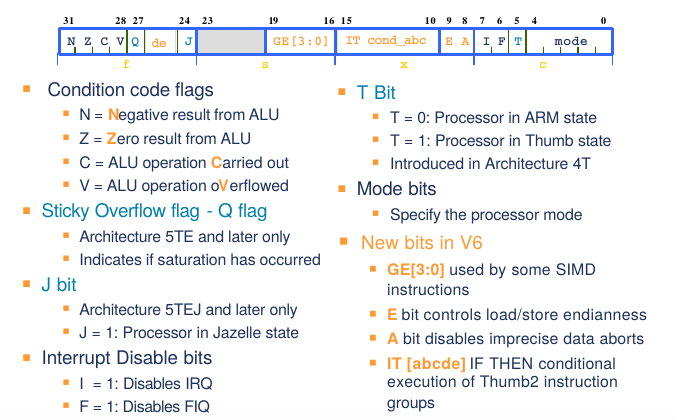
\includegraphics[width=.78\textwidth]{cpsr.pdf}
 \end{textblock*}
\end{frame}

\subsection{Registros}
\begin{frame}{Registros}
  \begin{textblock*}{\textwidth}(.3cm,1.2cm)
   \centering 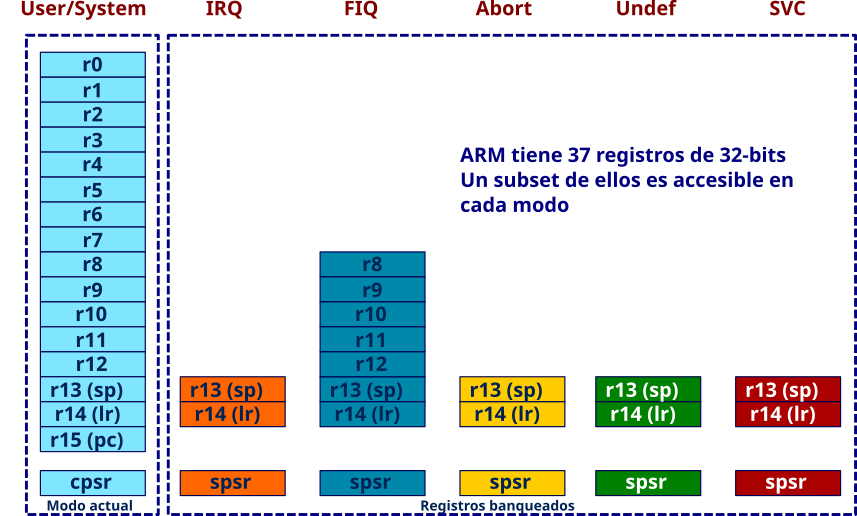
\includegraphics[width=.78\textwidth]{37Registros.pdf}
  \end{textblock*}
\end{frame}

\begin{frame}{Registros}
  \begin{textblock*}{\textwidth}(.3cm,1.2cm)
   \centering 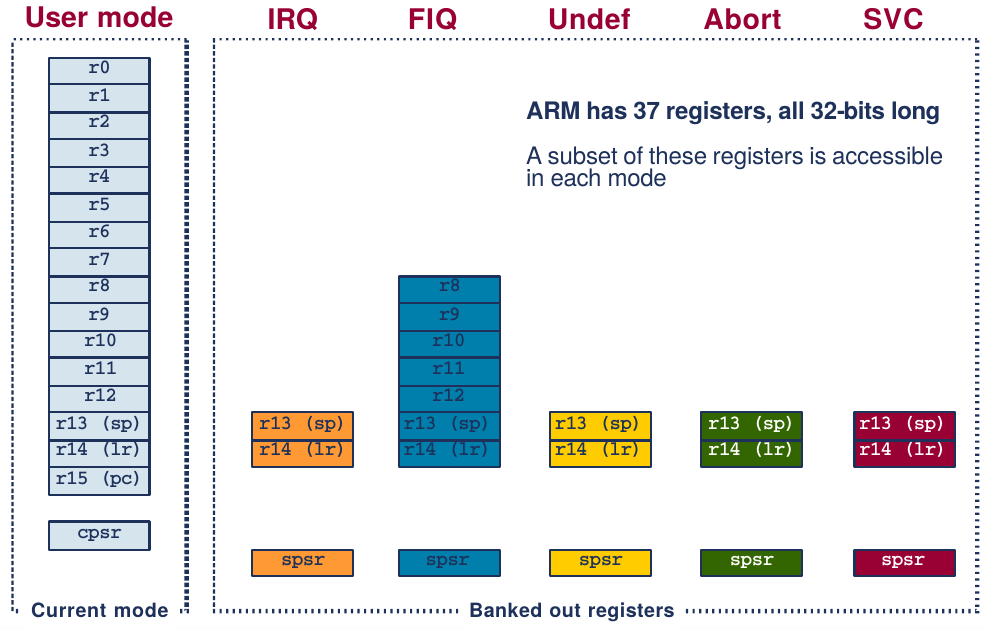
\includegraphics[width=.78\textwidth]{Registros.pdf}
  \end{textblock*}
\end{frame}

\end{document}
